Untuk mendukung fitur-fitur yang telah ditetapkan, dirancang basis data yang dapat menyimpan templat \textit{website}, informasi terkait jadwal sinkronisasi, serta metadata tambahan yang diperlukan dalam sistem. Berikut adalah rincian dari perancangan basis data generator konten \textit{website}:
\begin{enumerate}[label*=\arabic*.,ref=\arabic*]
    \item Entitas
    \begin{enumerate}[label=\arabic*.]
        \item Entitas \textit{user}: Pada entitas ini akan berisi informasi dari pengguna yang dapat mengakses sistem.

        \item Entitas \textit{db\_config}: Entitas ini berisi informasi konfigurasi koneksi ke basis data, termasuk \textit{host, port}, nama basis data, jenis basis data, dan kredensial. Entitas ini digunakan untuk mendukung operasi sinkronisasi data antara sistem dan basis data eksternal.

        \item Entitas \textit{website}: Entitas ini berisi informasi tentang \textit{website} yang dihasilkan oleh sistem, termasuk nama, direktori penyimpanan, dan pembuatnya.

        \item Entitas \textit{asset\_static}: Entitas ini berisi informasi tentang aset-aset statis seperti \textit{file} HTML, CSS, atau JavaScript yang digunakan dalam \textit{website}.

        \item Entitas \textit{asset\_dynamic}: Entitas ini berisi informasi tentang data dinamis yang digunakan untuk menggantikan \textit{placeholder} pada entitas \textit{asset\_static}.

        \item Entitas \textit{job}: Pada entitas ini akan berisi informasi tentang tugas sinkronisasi data, termasuk jadwal, konfigurasi sumber data, dan tujuan data. Entitas ini berfungsi untuk mengelola proses sinkronisasi otomatis antara basis data eksternal dan sistem.

    \end{enumerate}


    \item Atribut
    \begin{enumerate}[label=\arabic*.]
        \item Entitas \textit{user}
        \vspace{-0.5em}
        \begin{table}[H]
            \centering
            \begin{tabular}{|p{3.25cm}|p{8cm}|}
                \hline
                \rowcolor[HTML]{DAE8FC} 
                {\color[HTML]{000000} Nama Atribut} & {\color[HTML]{000000} Keterangan}           \\ \hline
                user\_id                           & Menyimpan \textit{primary key} bertipe \textit{integer} untuk setiap pengguna. \\ \hline
                username                           & Menyimpan nama pengguna bertipe \textit{varchar} dengan panjang maksimal 200 karakter dan bersifat unik. \\ \hline
                email                              & Menyimpan alamat email pengguna bertipe \textit{varchar} dengan panjang maksimal 200 karakter dan bersifat unik. \\ \hline
                password                           & Menyimpan kata sandi pengguna bertipe \textit{text} yang sudah dalam bentuk terenkripsi. \\ \hline
                created\_at                        & Menyimpan waktu pembuatan pengguna bertipe \textit{big integer} yang disimpan sebagai \textit{epoch unix time}. \\ \hline
                updated\_at                        & Menyimpan waktu pembaruan terakhir pengguna bertipe \textit{big integer} yang disimpan sebagai \textit{epoch unix time} dan dapat bernilai \textit{null}. \\ \hline
            \end{tabular}
            \caption{Atribut dan keterangan pada entitas user}
            \label{tab:user_entity}
        \end{table}

        \item Entitas \textit{website}
        \vspace{-0.5em}
        \begin{table}[H]
            \centering
            \begin{tabular}{|p{3.25cm}|p{8cm}|}
                \hline
                \rowcolor[HTML]{DAE8FC} 
                {\color[HTML]{000000} Nama Atribut} & {\color[HTML]{000000} Keterangan}           \\ \hline
                website\_id                        & Menyimpan \textit{primary key} bertipe \textit{integer} untuk setiap \textit{website}. \\ \hline
                created\_by                        & Menyimpan \textit{foreign key} ke entitas \textit{user}, bertipe \textit{integer}, menunjukkan pengguna yang membuat \textit{website}. \\ \hline
                updated\_by                        & Menyimpan \textit{foreign key} ke entitas \textit{user}, bertipe \textit{integer}, menunjukkan pengguna yang terakhir memperbarui \textit{website}. Nilai dapat \textit{null} jika belum pernah diperbarui. \\ \hline
                name                               & Menyimpan nama \textit{website} bertipe \textit{varchar} dengan panjang maksimal 200 karakter. \\ \hline
                dir\_path                          & Menyimpan direktori penyimpanan file website bertipe \textit{varchar} dengan panjang maksimal 200 karakter. \\ \hline
                created\_at                        & Menyimpan waktu pembuatan \textit{websit}e bertipe \textit{big integer} yang disimpan sebagai \textit{epoch unix time}. \\ \hline
                updated\_at                        & Menyimpan waktu pembaruan terakhir \textit{website} bertipe \textit{big integer} yang disimpan sebagai \textit{epoch unix time} dan dapat bernilai \textit{null}. \\ \hline
            \end{tabular}
            \caption{Atribut dan keterangan pada entitas website}
            \label{tab:website_entity}
        \end{table}

        \item Entitas db\_config
        \vspace{-0.5em}
        \begin{table}[H]
            \centering
            \begin{tabular}{|p{3.25cm}|p{8cm}|}
                \hline
                \rowcolor[HTML]{DAE8FC} 
                {\color[HTML]{000000} Nama Atribut} & {\color[HTML]{000000} Keterangan}           \\ \hline
                db\_config\_id                     & Menyimpan \textit{primary key} bertipe \textit{integer} untuk setiap konfigurasi basis data. \\ \hline
                created\_by                        & Menyimpan \textit{foreign key} ke entitas \textit{user}, bertipe \textit{integer}, menunjukkan pengguna yang membuat konfigurasi basis data. \\ \hline
                website\_id                        & Menyimpan \textit{foreign key} ke entitas \textit{website}, bertipe \textit{integer}, menunjukkan \textit{website} pemilik basis data. \\ \hline
                updated\_by                        & Menyimpan \textit{foreign key} ke entitas \textit{user}, bertipe \textit{integer}, menunjukkan pengguna yang terakhir memperbarui konfigurasi basis data. Nilai dapat \textit{null} jika belum pernah diperbarui. \\ \hline
                host                               & Menyimpan alamat \textit{host} basis data bertipe \textit{varchar} dengan panjang maksimal 200 karakter. \\ \hline
                port                               & Menyimpan port yang digunakan untuk koneksi basis data bertipe \textit{integer}. \\ \hline
                db\_name                           & Menyimpan nama basis data bertipe \textit{varchar} dengan panjang maksimal 200 karakter. \\ \hline
                user                               & Menyimpan nama pengguna untuk koneksi basis data bertipe \textit{varchar} dengan panjang maksimal 200 karakter. \\ \hline
                password                           & Menyimpan kata sandi untuk koneksi basis data bertipe TEXT. \\ \hline
                type                               & Menyimpan jenis basis data bertipe \textit{enum} (\textit{'mysql', 'postgresql'}). \\ \hline
                created\_at                        & Menyimpan waktu pembuatan konfigurasi basis data bertipe \textit{big integer} yang disimpan sebagai \textit{epoch unix time.} \\ \hline
                updated\_at                        & Menyimpan waktu pembaruan konfigurasi basis data terakhir bertipe \textit{big integer} yang disimpan sebagai \textit{epoch unix time} dan dapat bernilai \textit{null}. \\ \hline
            \end{tabular}
            \caption{Atribut dan keterangan pada entitas db\_config}
            \label{tab:db_config_entity}
        \end{table}

        \item Entitas asset\_static
        \vspace{-0.5em}
        \begin{table}[H]
            \centering
            \begin{tabular}{|p{3.25cm}|p{8cm}|}
                \hline
                \rowcolor[HTML]{DAE8FC} 
                {\color[HTML]{000000} Nama Atribut} & {\color[HTML]{000000} Keterangan}           \\ \hline
                asset\_static\_id                  & Menyimpan \textit{primary key} bertipe \textit{integer} untuk setiap aset statis. \\ \hline
                created\_by                        & Menyimpan \textit{foreign key} ke entitas \textit{user}, bertipe \textit{integer}, menunjukkan pengguna yang membuat aset. \\ \hline
                updated\_by                        & Menyimpan \textit{foreign key} ke entitas \textit{user}, bertipe \textit{integer}, menunjukkan pengguna yang terakhir memperbarui aset. Nilai dapat \textit{null} jika belum pernah diperbarui. \\ \hline
                website\_id                        & Menyimpan \textit{foreign key} ke entitas \textit{website}, bertipe \textit{integer}, menunjukkan \textit{website} tempat aset ini berada. \\ \hline
                parent\_id                         & Menyimpan \textit{foreign key} ke entitas \textit{asset\_static}, bertipe \textit{integer}, menunjukkan aset induk jika aset ini adalah bagian dari folder. Nilai dapat \textit{null}. \\ \hline
                name                               & Menyimpan nama aset bertipe \textit{varchar} dengan panjang maksimal 200 karakter. \\ \hline
                type                               & Menyimpan jenis aset bertipe \textit{enum} (\textit{'file', 'folder'}). \\ \hline
                content                            & Menyimpan konten aset bertipe \textit{text}. Nilai dapat \textit{null}. \\ \hline
                placeholders                       & Menyimpan definisi placeholder dalam format JSONB. Nilai dapat \textit{null}. \\ \hline
                created\_at                        & Menyimpan waktu pembuatan aset bertipe \textit{big integer} yang disimpan sebagai \textit{epoch unix time}. \\ \hline
                updated\_at                        & Menyimpan waktu pembaruan terakhir aset bertipe \textit{big integer} yang disimpan sebagai \textit{epoch unix time} dan dapat bernilai \textit{null}. \\ \hline
            \end{tabular}
            \caption{Atribut dan keterangan pada entitas asset\_static}
            \label{tab:asset_static_entity}
        \end{table}

        \item Entitas asset\_dynamic
        \vspace{-0.5em}
        \begin{table}[H]
            \centering
            \begin{tabular}{|p{3.25cm}|p{8cm}|}
                \hline
                \rowcolor[HTML]{DAE8FC} 
                {\color[HTML]{000000} Nama Atribut} & {\color[HTML]{000000} Keterangan}           \\ \hline
                asset\_dynamic\_id                 & Menyimpan \textit{primary key} bertipe \textit{integer} untuk setiap aset dinamis. \\ \hline
                created\_by                        & Menyimpan \textit{foreign key} ke entitas \textit{user}, bertipe \textit{integer}, menunjukkan pengguna yang membuat aset dinamis. \\ \hline
                updated\_by                        & Menyimpan \textit{foreign key} ke entitas \textit{user}, bertipe \textit{integer}, menunjukkan pengguna yang terakhir memperbarui aset dinamis. Nilai dapat \textit{null} jika belum pernah diperbarui. \\ \hline
                asset\_static\_id                  & Menyimpan \textit{foreign key} ke entitas \textit{asset\_static}, bertipe \textit{integer}, menunjukkan aset statis yang terkait. \\ \hline
                placeholder\_values                & Menyimpan nilai pengganti untuk \textit{placeholder} dalam format JSONB. \\ \hline
                created\_at                        & Menyimpan waktu pembuatan aset dinamis bertipe \textit{big integer} yang disimpan sebagai \textit{epoch unix time}. \\ \hline
                updated\_at                        & Menyimpan waktu pembaruan terakhir aset dinamis bertipe \textit{big integer} yang disimpan sebagai \textit{epoch unix time} dan dapat bernilai \textit{null}. \\ \hline
            \end{tabular}
            \caption{Atribut dan keterangan pada entitas asset\_dynamic}
            \label{tab:asset_dynamic_entity}
        \end{table}

        \item Entitas job
        \vspace{-0.5em}
        \begin{table}[H]
            \centering
            \begin{tabular}{|p{3.25cm}|p{8cm}|}
                \hline
                \rowcolor[HTML]{DAE8FC} 
                {\color[HTML]{000000} Nama Atribut} & {\color[HTML]{000000} Keterangan}           \\ \hline
                job\_id                            & Menyimpan \textit{primary key} bertipe \textit{integer} untuk setiap tugas sinkronisasi. \\ \hline
                created\_by                        & Menyimpan \textit{foreign key} ke entitas \textit{user}, bertipe \textit{integer}, menunjukkan pengguna yang membuat tugas sinkronisasi. \\ \hline
                updated\_by                        & Menyimpan \textit{foreign key} ke entitas \textit{user}, bertipe \textit{integer}, menunjukkan pengguna yang terakhir memperbarui tugas sinkronisasi. Nilai dapat \textit{null} jika belum pernah diperbarui. \\ \hline
                db\_config\_id                     & Menyimpan \textit{foreign key} ke entitas \textit{db\_config}, bertipe \textit{integer}, menunjukkan konfigurasi basis data terkait. \\ \hline
                name                               & Menyimpan nama \textit{job}, bertipe \textit{varchar} dengan panjang maksimal 100 karakter. \\ \hline
                cron                               & Menyimpan format cron untuk penjadwalan tugas bertipe \textit{varchar} dengan panjang maksimal 20 karakter. \\ \hline
                count                               & Menyimpan jumlah \textit{job} yang sudah dijalankan bertipe \textit{integer}. \\ \hline
                tables                             & Menyimpan daftar tabel sumber dalam, bertipe JSONB. \\ \hline
                endpoint                           & Menyimpan URL API tujuan sinkronisasi bertipe \textit{varchar} dengan panjang maksimal 500 karakter. \\ \hline
                headers                            & Menyimpan header yang diperlukan untuk API tujuan dalam, bertipe JSONB. \\ \hline
                request\_format                    & Menyimpan format \textit{request} ke API tujuan dalam, bertipe JSONB. \\ \hline
                transform                          & Menyimpan aturan pemetaan antara data hasil ekstraksi dan struktur data yang diharapkan oleh API tujuan, bertipe JSONB. \\ \hline
                last\_run                          & Menyimpan waktu eksekusi terakhir, bertipe \textit{big integer} yang disimpan sebagai epoch unix time. Nilai dapat \textit{null} jika belum pernah dieksekusi. \\ \hline
                next\_run                          & Menyimpan waktu eksekusi berikutnya, bertipe \textit{big integer} yang disimpan sebagai epoch unix time. \\ \hline
                created\_at                        & Menyimpan waktu pembuatan tugas sinkronisasi bertipe \textit{big integer} yang disimpan sebagai epoch unix time. \\ \hline
                updated\_at                        & Menyimpan waktu pembaruan terakhir tugas sinkronisasi bertipe \textit{big integer} yang disimpan sebagai epoch unix time dan dapat bernilai \textit{null}. \\ \hline
            \end{tabular}
            \caption{Atribut dan keterangan pada entitas job}
            \label{tab:job_entity}
        \end{table}

\end{enumerate}


    \item Rancangan Entity Relationship Diagram (ERD)
        \begin{figure}[H]
            \centering
            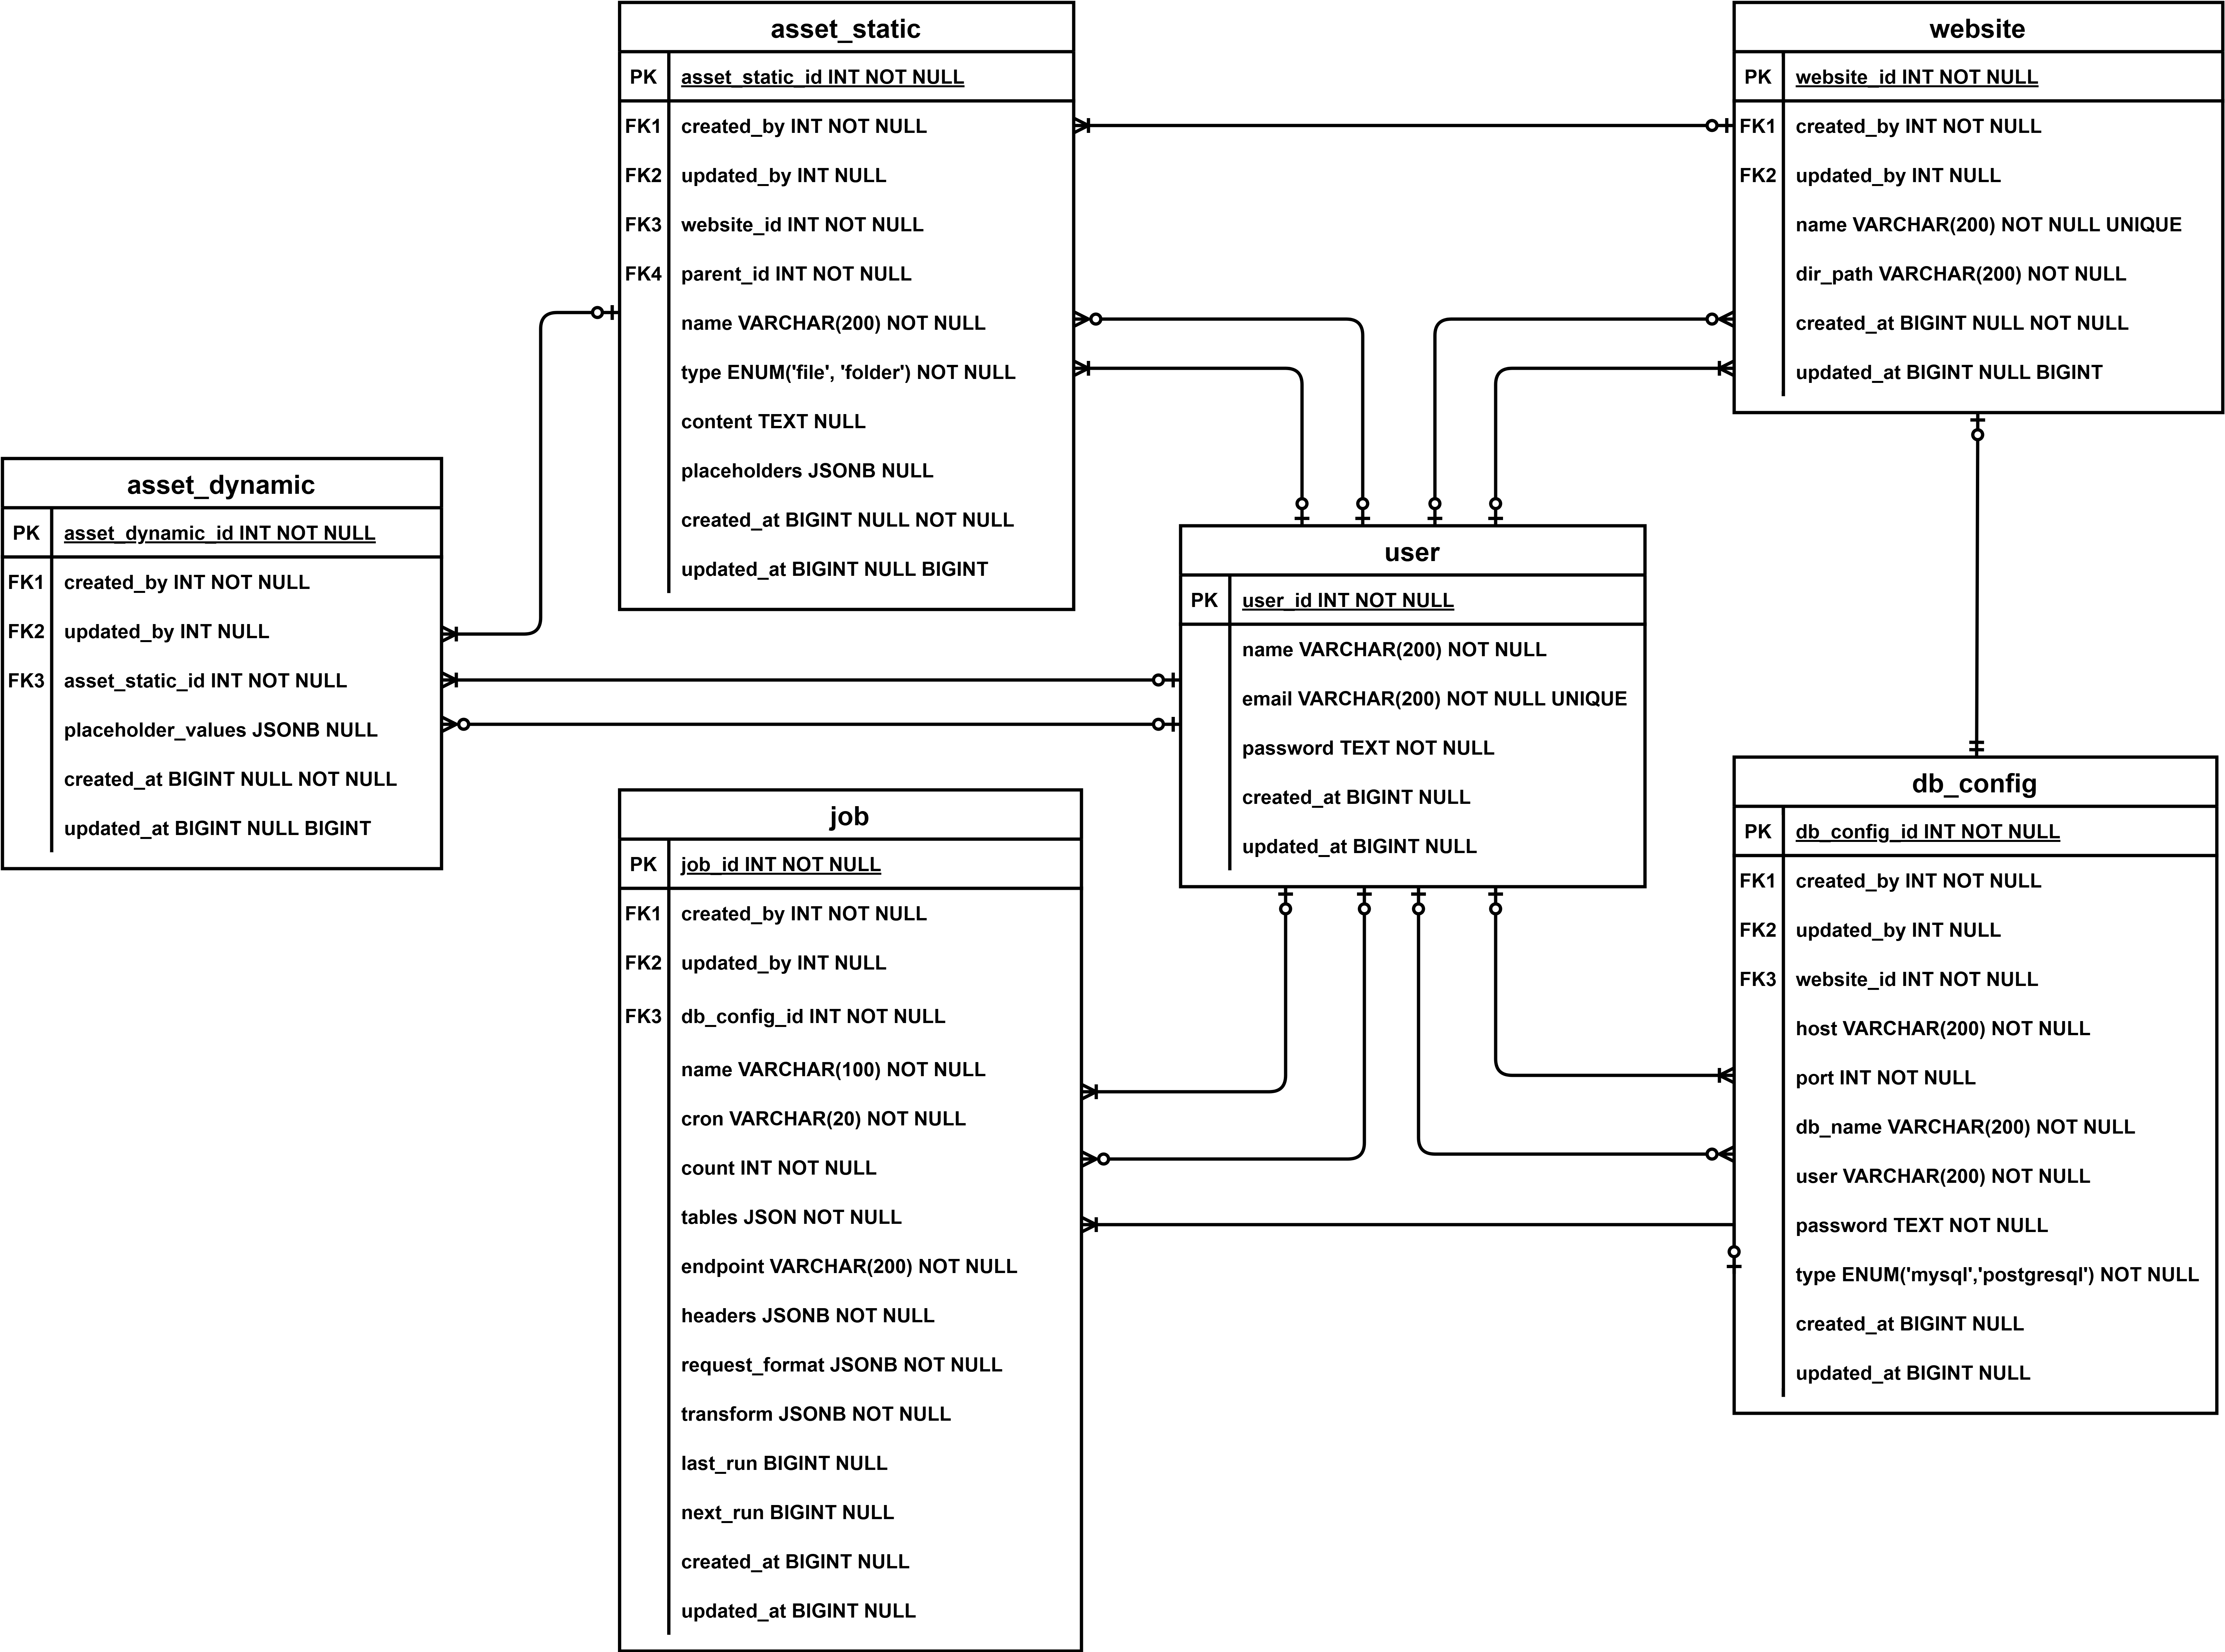
\includegraphics[width=0.8\linewidth]{figures/ERD-10.png}
            \caption{ERD Basis Data Templat}
            \label{fig:ERD-GeneratorKontenWebsite}
        \end{figure}

\end{enumerate}